\section{Durchführung}
\label{sec:Durchführung}




\begin{figure}[H]
    \centering
    \caption{}
    \begin{subfigure}{0.48\textwidth}
      \centering
      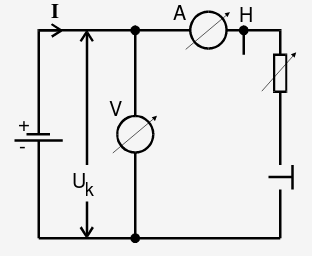
\includegraphics[width=\linewidth-60pt,height=\textheight-60pt,keepaspectratio]{content/Spannungsquelle2.png}
      \caption{\footnotesize Messungaufbau zur $U_0$ und $R_i$-Bestimmung [1]}
      \label{fig:Spannung2}
    \end{subfigure}
    \begin{subfigure}{0.48\textwidth}
      \centering
      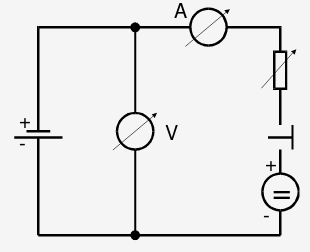
\includegraphics[width=\linewidth-60pt,height=\textheight-60pt,keepaspectratio]{content/Spannungsquelle3.png}
      \caption{\footnotesize $U_0$ und $R_i $-Bestimmung mit Gegenspannung}
      \label{fig:Spannung3}
    \end{subfigure}
  \end{figure}


    Zunächst wird die Leerlauflaufspannung einer Monozelle ermittelt. Hierfür
     wird die Monozelle direkt and den Voltmeter Ein- bzw. Ausgang eines
      Multimeters angeschlossen. Aufgrund des hohen Innenwiderstandes des Voltmeters
       lässt sich die Leerlaufspannung durch die Klemmenspannung nähern. Zur besseren
        Untersuchung wird auch der Innenwiderstand des Voltmeters notiert.

Im Anschluss wird die Klemmenspannung $U_k$ in Abhängigkeit des Belastungsstromes I gemessen.
 Hierzu wird die Schaltung nach Abb. 2(a) verwendet. Volt und Amperemeter werden wieder durch
  durch die jeweiligen Modi zweier Multimeter realisiert. Um den Belastungsstrom
   zu ändern, wird ein einstellbarer Widerstand $R_a$ eingesetzt, welcher im bereich von
    $0-\SI{50}{\ohm}$ variiert wird. Das gleiche Verfahren wird nochmals mit dem Sinus- bzw.
    dem Rechteckausgang eines RC-generators durchgeführt. Für die Variationsbereiche
     der dort eingesetzten Widerstände gilt:
     $\SI{1}{V}$-Sinusausgang: $R_a \in [0,1 -\SI{5}{\kilo\ohm}]$\\
     $\SI{1}{V}$-Rechteckausgang: $R_a \in [20 -\SI{250}{\ohm}]$\\
     
Es ist zu beachten, dass die Multimeter nur für einen engen Frequenzbereich des
 Wechselstromes geeicht sind. Zuletzt wird das voherige Verfahren an einer Monozelle
  unter Anschluss einer Gegenspannung betrachtet. Hierzu wird eine Gegenspannung
   wie in Abb.(b) in den Stromkreis eingeschlossen, welche ca $\SI{2}{V}$ größer als
   $U_0$ ist. Der Strom fließt nun in umgekehrter Richtung, wodurch gilt:
   \begin{equation}
     U_k = U_0 + IR_i
     \end{equation}
